\documentclass[12pt]{exam}
\usepackage{amsmath}
\usepackage{amssymb}
\usepackage{graphicx}
\usepackage{enumitem}
\usepackage{amsfonts}
\usepackage{amssymb}
\usepackage{ifthen}
\usepackage{geometry}
\noprintanswers

\usepackage{tikz}
\usetikzlibrary{shapes,backgrounds}
\newcommand*\circled[1]{\tikz[baseline=(char.base)]{
    \node[shape=circle, draw, inner sep=1pt, 
        minimum height=12pt] (char) {#1};}}

\usepackage{framed}

\addtolength{\textheight}{4.5cm}
\addtolength{\topmargin}{-1.3cm}
\addtolength{\textwidth}{3.5cm}
\addtolength{\oddsidemargin}{-2cm}
\addtolength{\evensidemargin}{-2cm}
\setlength\parindent{0pt}

\newcommand {\DS} [1] {${\displaystyle #1}$}
\newcommand{\vv}{\vspace{.1cm}}

\newcommand{\R}{\mathbb{R}}
\newcommand{\Q}{\mathbb{Q}}
\newcommand{\Z}{\mathbb{Z}}
\newcommand{\N}{\mathbb{N}}

\pagestyle{empty}


%============================================
%137 COLOUR PALETTE
%============================================

\definecolor{137cp1}{RGB}{13, 33, 161}
\definecolor{137cp2}{RGB}{51, 161, 253}
\definecolor{137cp3}{RGB}{255, 67, 101}
\definecolor{137cp4}{RGB}{232, 144, 5}

% to use colours easily
\newcommand{\azul}[1]{{\color{blue} #1}}
\newcommand{\rojo}[1]{{\color{red} #1}}
 
% box in red and blue in math and outside of math
\newcommand{\cajar}[1]{\boxed{\mbox{\rojo{ #1}}}}
\newcommand{\majar}[1]{\boxed{\rojo{ #1}}}
\newcommand{\cajab}[1]{\boxed{\mbox{\azul{ #1}}}}
\newcommand{\majab}[1]{\boxed{\azul{ #1}}}

%============================================
%HYPERLINKS
%============================================

\usepackage{hyperref}
\hypersetup{colorlinks}
\hypersetup{urlcolor=137cp3, linkcolor=137cp1}

%============================================
%Commands used only for this file
%============================================


%%%%%%%%%%%%%%%%%%%%%%%%%%%%%%%%%%%%%%%%%


\begin{document}

{\large
	\begin{center}
		{\bf MAT 137Y: Calculus with proofs}\\
		{\bf Assignment 5} \\
		{\bf Due on Sunday, December 20 by 11:59pm via Crowdmark}
	\end{center}
}

\vv

\begin{quotation}
{\bf Instructions:}
	\begin{itemize}
		\item	 You will need to submit your solutions electronically via Crowdmark.   \href{https://www.math.toronto.edu/~alfonso/137/PS/137_CM.html}{See MAT137 Crowdmark help page for instructions}.  Make sure you understand how to submit and that you try the system ahead of time.  If you leave it for the last minute and you run into technical problems, you will be late.  There are no extensions for any reason.
		\item You may submit individually or as a team of two students.  See the link above for more details.
		\item  You will need to submit your answer to each question separately.
		\item  This problem set is about Unit 6.
	\end{itemize}
\end{quotation}
\vv

\begin{enumerate}

\item Every morning Neo packs his backpack and walks a distance $L$ through a straight path in the forest from his home ($A$) to the unicorn sanctuary ($B$).  One day he discovers someone has built an electric fence in the exact middle of his daily path (the dashed, red line in the picture):
\begin{center}
\begin{tikzpicture}
	\draw (0,0) to (6,0);
	\draw[red, very thick, dashed] (3,-1) to (3,1);
	\draw[fill] (0,0) circle [radius=.1];
	\draw[fill] (6,0) circle [radius=.1];
	\node[xshift=-10pt] at (0,0) {$A$} ;
	\node[xshift= 10pt] at (6,0) {$B$} ;
\end{tikzpicture}
\end{center}
The fence has length $2b$ --  it extends for a distance $b$ on each side of the path -- and is perpendicular to the path.  After a few days, Neo notices that the electric fence is turned on only half the time, but he does not know if the fence is on or off on any given day until he walks up to it and throws his cat at the fence to test it.  If the fence is off, he can just quickly climb over it.  Otherwise, he has to walk around it.  He devises a plan: he will walk straight from his home to some point $P$ in the fence; then, he will walk around it or climb over it depending on whether the fence is on or off.    Which point $P$ should he choose in order to minimize the \emph{average} length of his trip?


\vv

\emph{Proof:}

\vv

\begin{center}
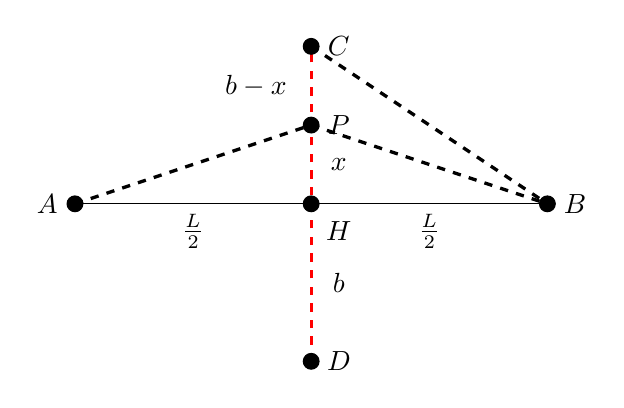
\begin{tikzpicture}
	\draw (0,0) to (6,0);
	\draw[red, very thick, dashed] (3,-2) to (3,2);
	\draw[very thick, dashed] (0,0) to (3,1);
	\draw[very thick, dashed] (3,1) to (6,0);
	\draw[very thick, dashed] (3,2) to (6,0);
	\draw[fill] (0,0) circle [radius=.1];
	\draw[fill] (6,0) circle [radius=.1];
	\draw[fill] (3,0) circle [radius=.1];
	\draw[fill] (3,2) circle [radius=.1];
	\draw[fill] (3,1) circle [radius=.1];
	\draw[fill] (3,-2) circle [radius=.1];
	\node[xshift=-10pt] at (0,0) {$A$} ;
	\node[yshift=-10pt] at (1.5,0) {$\frac{L}{2}$} ;
	\node[yshift=-10pt] at (4.5,0) {$\frac{L}{2}$} ;
	\node[xshift= 10pt] at (6,0) {$B$} ;
	\node[xshift= 10pt] at (3,2) {$C$} ;
	\node[xshift= -20pt] at (3,1.5) {$b-x$} ;
	\node[xshift= 10pt] at (3,1) {$P$} ;
	\node[xshift= 10pt] at (3,0.5) {$x$} ;
	\node[xshift= 10pt] at (3,-1) {$b$} ;
	\node[xshift= 10pt] at (3,-2) {$D$} ;
	\node[xshift= 10pt, yshift= -10pt] at (3,0) {$H$} ;
\end{tikzpicture}
\end{center}

By the assumption of the question, we know line segment $AB=L$ and the fence length is $2b$. We set point $C$ as upper endpoint of fence and $D$ as lower endpoint, then line segment $CD=2b$. Set point $H$ at where line segment $AB$ and fence $CD$ intersect. Then by assumption `electric fence in the exact middle of his daily path` and `it extends for a distance $b$ on each side of the path`, we know $AH=BH=\frac{L}{2}$ and $CH=DH=b$. We set point $P$ on the $CH$ to calculate length of the trip since point $P$ can be reflected by $AB$. Suppose $PH=x$ and we can get $CP=CH-PH=b-x$.

By Pythagoras Theorem, we know:
\begin{align*}
    PB=AP&=\sqrt{AH^2+PH^2} \quad(\mbox{Pythagoras Theorem})\\
    &=\sqrt{(\frac{L}{2})^2+x^2} \qquad \mbox{ for some } x\in[0,b] \quad(AH=\frac{L}{2} \mbox{ and } PH=x)
\end{align*}

By Pythagoras Theorem, we also know:
\begin{align*}
    BC&=\sqrt{CH^2+HB^2} \quad(\mbox{Pythagoras Theorem})\\
    &=\sqrt{b^2+(\frac{L}{2})^2}\quad(BH=\frac{L}{2} \mbox{ and } PH=b)
\end{align*}

If the electric fence is on, the length of the trip is:
\begin{align*}
    AP+PC+BC
    &=\sqrt{(\frac{L}{2})^2+x^2}+(b-x)+\sqrt{b^2+(\frac{L}{2})^2} \quad \mbox{ for some } x\in[0,b] \quad \circled{1}\\ &\quad(AP=\sqrt{(\frac{L}{2})^2+x^2}\mbox{ and }PC=b-x\mbox{ and }BC=\sqrt{b^2+(\frac{L}{2})^2})
\end{align*}

If the electric fence is off, the length of the trip is:
\begin{align*}
    AP+PB&=2AP \quad(AP=PB)\\
    &=2\sqrt{(\frac{L}{2})^2+x^2} \qquad \mbox{ for some } x\in[0,b] \quad(AP=\sqrt{(\frac{L}{2})^2+x^2}) \quad \circled{2}
\end{align*}

Then the average length represented by $f$ of the trip is:
\begin{align*}
    f(x)&=\frac{AP+PC+BC+AP+PB}{2}\\
    &=\frac{\sqrt{(\frac{L}{2})^2+x^2}+(b-x)+\sqrt{b^2+(\frac{L}{2})^2}+2\sqrt{(\frac{L}{2})^2+x^2}}{2} \quad\mbox{Total length is }\mbox{\circled{1} and \circled{2}}\\
    &=\frac{3\sqrt{(\frac{L}{2})^2+x^2}}{2}+\frac{b-x}{2}+\frac{\sqrt{b^2+(\frac{L}{2})^2}}{2} \quad\circled{3}
\end{align*}

Since the terms under square root are equal to or bigger than $0$, so $f$ are strictly positive and continuous on $[0,b]$. By Extreme Value Theorem, we know $f$ has a minimum on $[0,b]$, which we know must be a critical point or at an endpoint of the domain. $f$ is differentiable on $(0,b)\subseteq[0,b]$ and by implicit differentiation and \circled{3}, we want to find critical point:
\begin{align*}
    f'(x)
    &=\frac{3}{2}\cdot\frac{2x}{2\sqrt{(\frac{L}{2})^2+x^2}}-\frac{1}{2} \quad(\mbox{Chain Rule and Implicit Differentiation})\\
    &=\frac{3x}{2\sqrt{(\frac{L}{2})^2+x^2}}-\frac{1}{2}\\
\end{align*}
We want to find critical point, so we should let $f'(x) = 0$, which implies:
\begin{align*}
    \frac{3x}{2\sqrt{(\frac{L}{2})^2+x^2}}&=\frac{1}{2}\\
    3x&=\sqrt{(\frac{L}{2})^2+x^2}\\
    9x^2&=(\frac{L}{2})^2+x^2\\
    8x^2&=(\frac{L}{2})^2\\
    x&=\frac{\sqrt{2}}{8}L
\end{align*}

Since $x > 0$, the only critical point is $x=\frac{\sqrt{2}}{8}L$.

The table shows that $f$ is decreasing on the left side of critical point and $f$ is increasing on the right side of critical point. So $x=\frac{\sqrt{2}}{8}L$ is a local minimum.

\begin{tabular}{l|l|l|l}
\hline
$x$     & $0$            & $\frac{\sqrt{2}}{8}L$ & $L$                               \\
\hline
$f'(x)$ & $-\frac{1}{2}$ & $0$                   & $\frac{3\sqrt{5}}{5}-\frac{1}{2}$
\end{tabular}

However we know $x\in[0,b]$, we don't know the relationship between $L$ and $b$.

The answer should be splitted in to cases:
\begin{itemize}
    \item If $x=\frac{\sqrt{2}}{8}L\in [0,b]$, then point $P$ is $\frac{\sqrt{2}}{8}L$ up or down of point $H$.
    \item If $x=\frac{\sqrt{2}}{8}L>b$, since $f$ is decreasing when $x=\frac{\sqrt{2}}{8}L$, the minimum then is at $x=b$ as point $P$ is at $C$ or $D$.
    \item $x=\frac{\sqrt{2}}{8}L$ will never less than $0$ since $L>0$.
\end{itemize}

\newpage

\item  
	\begin{enumerate}
				
		\item  Let $f$ be a function with domain $\R$.  Assume $f$ has derivatives of every order.  Find all possible real numbers $A, B, C \in \R$ such that
			\begin{equation} \label{eq:ABC}
				\lim_{x \to 0} \frac{f(x) - \left[ Ax^2 + B x + C \right]}{x^2} = 0.
			\end{equation}	
			
			\emph{Note:} In your answer, $A$, $B$ and $C$ will depend on values of $f$ and its derivatives.  We are asking for \emph{all} possible answers.  We want you to prove that your choices of $A$, $B$, and $C$ satisfy \eqref{eq:ABC}, and that there are no other choices that satisfy \eqref{eq:ABC}.
			
			
		\item  Let $f$ be a function with domain $\R$.  Assume $f$ has derivatives of every order.   Let $N$ be a positive integer.  Find a polynomial \DS{P_N} such that
			$$
				\lim_{x \to 0} \frac{f(x) - P_N(x)}{x^N} = 0
			$$
			\emph{Suggestion:} You may want to do some rough work until you can form a conjecture.    Do not submit the rough work.  To prove your conjecture, use induction.
		\item  Using your new result, find polynomials $P$  and $Q$ such that
			$$
				\lim_{x \to 0} \frac{e^x - P(x)}{x^6} = 0, \quad \quad \lim_{x \to 0} \frac{\sin x - Q(x)}{x^{11}} = 0.
			$$
	\end{enumerate}

\vv

\item  In Video 6.13, you learned about various geometrical notions that we could have used to define concavity.  Here is yet another one.

 Let $f$ be a function defined on an interval $I$.  Given two points $P$ and $Q$ on the graph of $f$, we will call $m_{P,Q}$ the slope of the line going through $P$ and $Q$.  We say that the function $f$ is ``cave up" on $I$ when for every 3 different points $P$, $Q$, and $R$ on the graph of $f$, if $P$ is to the left of $Q$, and $Q$ is to the left of $R$, then $m_{P,Q} < m_{Q,R}$.  Sketch a graph and make sure you understand this definition geometrically  before continuing.
 
 Assume $f$ is differentiable on $I$. 
		Prove that IF $f$ is concave up on $I$, THEN $f$ is cave up on $I$.


\emph{Hint:}  Use MVT.

\emph{Note:}  It is also possible to prove that cave up implies concave up, but we will skip it for now.  In fact, all of the different versions of concavity you have learned are equivalent for differentiable functions.	

\vv

\item  Let's recall the definition of horizontal/slant asymptote.  Let $f$ be a function defined at least on an interval $(c,\infty)$ for some $c \in \R$.
We say that $f$ has an asymptote as $x \to \infty$ when there exist numbers $m, b \in \R$ such that
	$$	
		\lim_{x \to \infty} \left[ f(x) - \left( mx + b \right) \right] \; = \; 0.
	$$
Notice that this includes both slant asymptotes (when $m \neq 0$) and horizontal asymptotes (when $m =0$).
	
Consider the following two claims:	
			\begin{center}
				{\bf Claim A:} \quad \quad
					IF $f$ has an asymptote as $x \to \infty$,  \quad
					THEN \DS{\lim_{x \to \infty} \frac{f(x)}{x}} exists.
				
				{\bf Claim B:} \quad \quad 		
					IF \DS{\lim_{x \to \infty} \frac{f(x)}{x}} exists, \quad
					THEN $f$ has an asymptote as $x \to \infty$.
			\end{center}
	\begin{enumerate}
		\item Prove that Claim A is true.
		\item Prove that Claim B is false.

		\item  Here is one more false claim and a bad proof.
			\begin{quotation}
				\noindent
				{\bf Claim C:} Assume the function $f$ is differentiable and that \DS{\lim_{x \to \infty} f(x) = \infty}.
				
				$$  \lim_{x \to \infty} \frac{f(x)}{x} \mbox{ exists} \quad \iff \quad \lim_{x \to \infty} f'(x) \mbox{ exists } $$
				
				
				\noindent
				{\bf ``Proof":}  We can use L'H\^{o}pital's Rule:
					$$
						\lim_{x \to \infty} \frac{f(x)}{x} \; = \; \lim_{x \to \infty} \frac{\frac{d}{dx} f(x)}{\frac{d}{dx} x} 
							\; = \; \lim_{x \to \infty} \frac{f'(x)}{1} \; = \; \lim_{x \to \infty} f'(x)
					$$
					\ \hfill $\square$
			\end{quotation}
			Explain the  error in the proof.
			
			Then prove that the claim is false with a counterexample.
	\end{enumerate}

\end{enumerate}


\end{document}

%%%%%%%%%%%%%%%%%%%%%%%%%%%%%%%%%%%%%%%
%%%%%%%%%%%%%%%%%%%%%%%%%%%%%%%%%%%%%%%
%%%%%%%%%%%%%%%%%%%%%%%%%%%%%%%%%%%%%%%


	
